
\section{Analysis}
\label{sec:analysis}

The main goal of the analysis is to estimate the source-count distribution of stars in the
images by predicting their magnitudes. I fitted a model to the input image, which can be
used by the user to predict the magnitudes of stars in other images. To train the
predictor, I needed to obtain the true magnitudes of stars in the input image. This
process involves multiple steps, that can be used independently. The first step finds the
pixel coordinates of each star in the image (\autoref{sec:star-identification}). These are
mapped to the celestial sphere to find the corresponding right ascension and declination
(\autoref{sec:pixel-to-sky-mapping}). The true magnitudes are obtained by matching the
sky coordinates to stars in the SIMBAD database (\autoref{sec:catalog-matching}). The
model is then fitted to the labeled list of stars (\autoref{sec:magnitude-estimation}).
Finally, the distribution of predicted magnitudes is compared to the literature
(\autoref{sec:source-count-distribution}).

\subsection{Star Identification}
\label{sec:star-identification}

\begin{figure}[tb]
  \centering
  \begin{subfigure}{.33\textwidth}
    \centering
    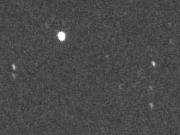
\includegraphics[width=\linewidth]{floodFill_original.png}
    \caption{Cutout of the input image}
    \label{fig:floodfill-original}
  \end{subfigure}%
  \hfill
  \begin{subfigure}{.33\textwidth}
    \centering
    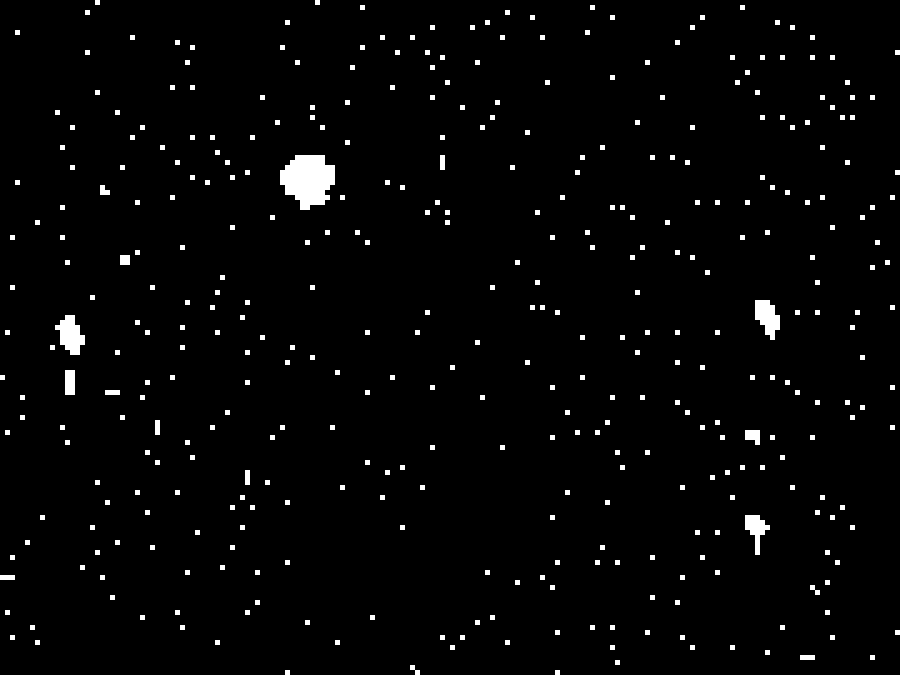
\includegraphics[width=\linewidth]{floodFill_before_erode.png}
    \caption{Mask after \texttt{floodFill} method}
    \label{fig:floodfill}
  \end{subfigure}%
  \hfill
  \begin{subfigure}{.33\textwidth}
    \centering
    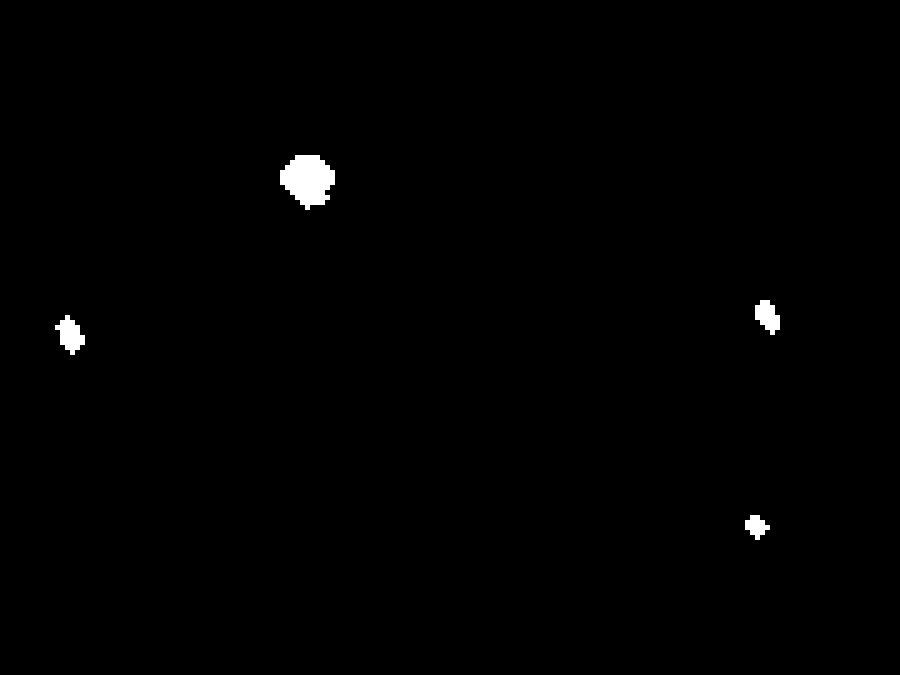
\includegraphics[width=\linewidth]{floodFill_after_erode.png}
    \caption{Mask after Opening operation}
    \label{fig:opening}
  \end{subfigure}
  \caption{}
  \label{fig:star-identification}
\end{figure}

Starting from the calibrated image, we need to identify the stars in the image. First,
we classify each pixel as belonging to a star or the background. A fast and simple
approach is the \texttt{cv2.floodFill} method from the OpenCV library \cite{opencv2000}.
It starts at a seed pixel, fills all connected pixels with a similar intensity and returns
the mask of the filled area. A pixel $(x, y)$ with a value $\texttt{src}(x, y)$ is
considered to have a similar intensity iff
\begin{align*}
  \texttt{src}(x', y') - \texttt{loDiff} \leq \texttt{src}(x, y) \leq \texttt{src}(x', y') + \texttt{upDiff},
\end{align*}
where $\texttt{src}(x', y')$ is the value of one of the neighboring pixels that is already
filled and \texttt{loDiff} and \texttt{upDiff} are thresholds set by the user. This rule
is applied iteratively to all pixels. To fill the background of the input image, I
chose the darkest pixel as the seed and set $\texttt{loDiff} = \infty$ and
$\texttt{upDiff} = 5$ (for an 8-bit image). A lower value of \texttt{upDiff} would result
in too much noise being classified as stars, while a higher value would miss faint stars.
The result is shown in \autoref{fig:floodfill}. We can see that there are many single
pixels of noise not being classified as background. To remove them, I applied the
morphological operation Opening with a $3 \times 3$ kernel using the
\texttt{cv2.morphologyEx} method from OpenCV. This operation erodes the image and then
dilates it, which removes objects that are at most two pixels wide. All other components
are preserved. The result is shown in \autoref{fig:opening}. Finally, I used the
\texttt{cv2.connectedComponents} method to separate the objects in the mask. I defined the
center of the bounding box of each object as the pixel coordinates of the star it
corresponds to.

In the calibrated image, the method identified 1001 stars. According to the SIMBAD
database, there are 746 stars with a visible magnitude of less than 7.0 and 2330 stars
with a magnitude less than 8.0 in the field of view of the image. The ADQL query used to
obtain this number is given in \autoref{lst:simbad-query}. If two stars are very close
together, the method might classify them as one object. During visual inspection however,
I only found two cases of this happening. Stars not being recognized is more commonly due
to them being too faint to distinguish them from noise. \autoref{fig:removing-stars} shows
histograms of the calibrated image before and after removing the stars identified by this
method. In \autoref{fig:after-removing-stars} we can see that almost all pixels identified
as background have a relative value of at most $20\%$.

I also tested other approaches, like template matching. The main problem was to define a
general template for stars, that would fit different sizes and brightnesses. This drawback
made template matching much more complex and less reliable than the flood fill method.

\begin{figure}[tb]
  \centering
  % \begin{subfigure}{.33\textwidth}
  %   \centering
  %   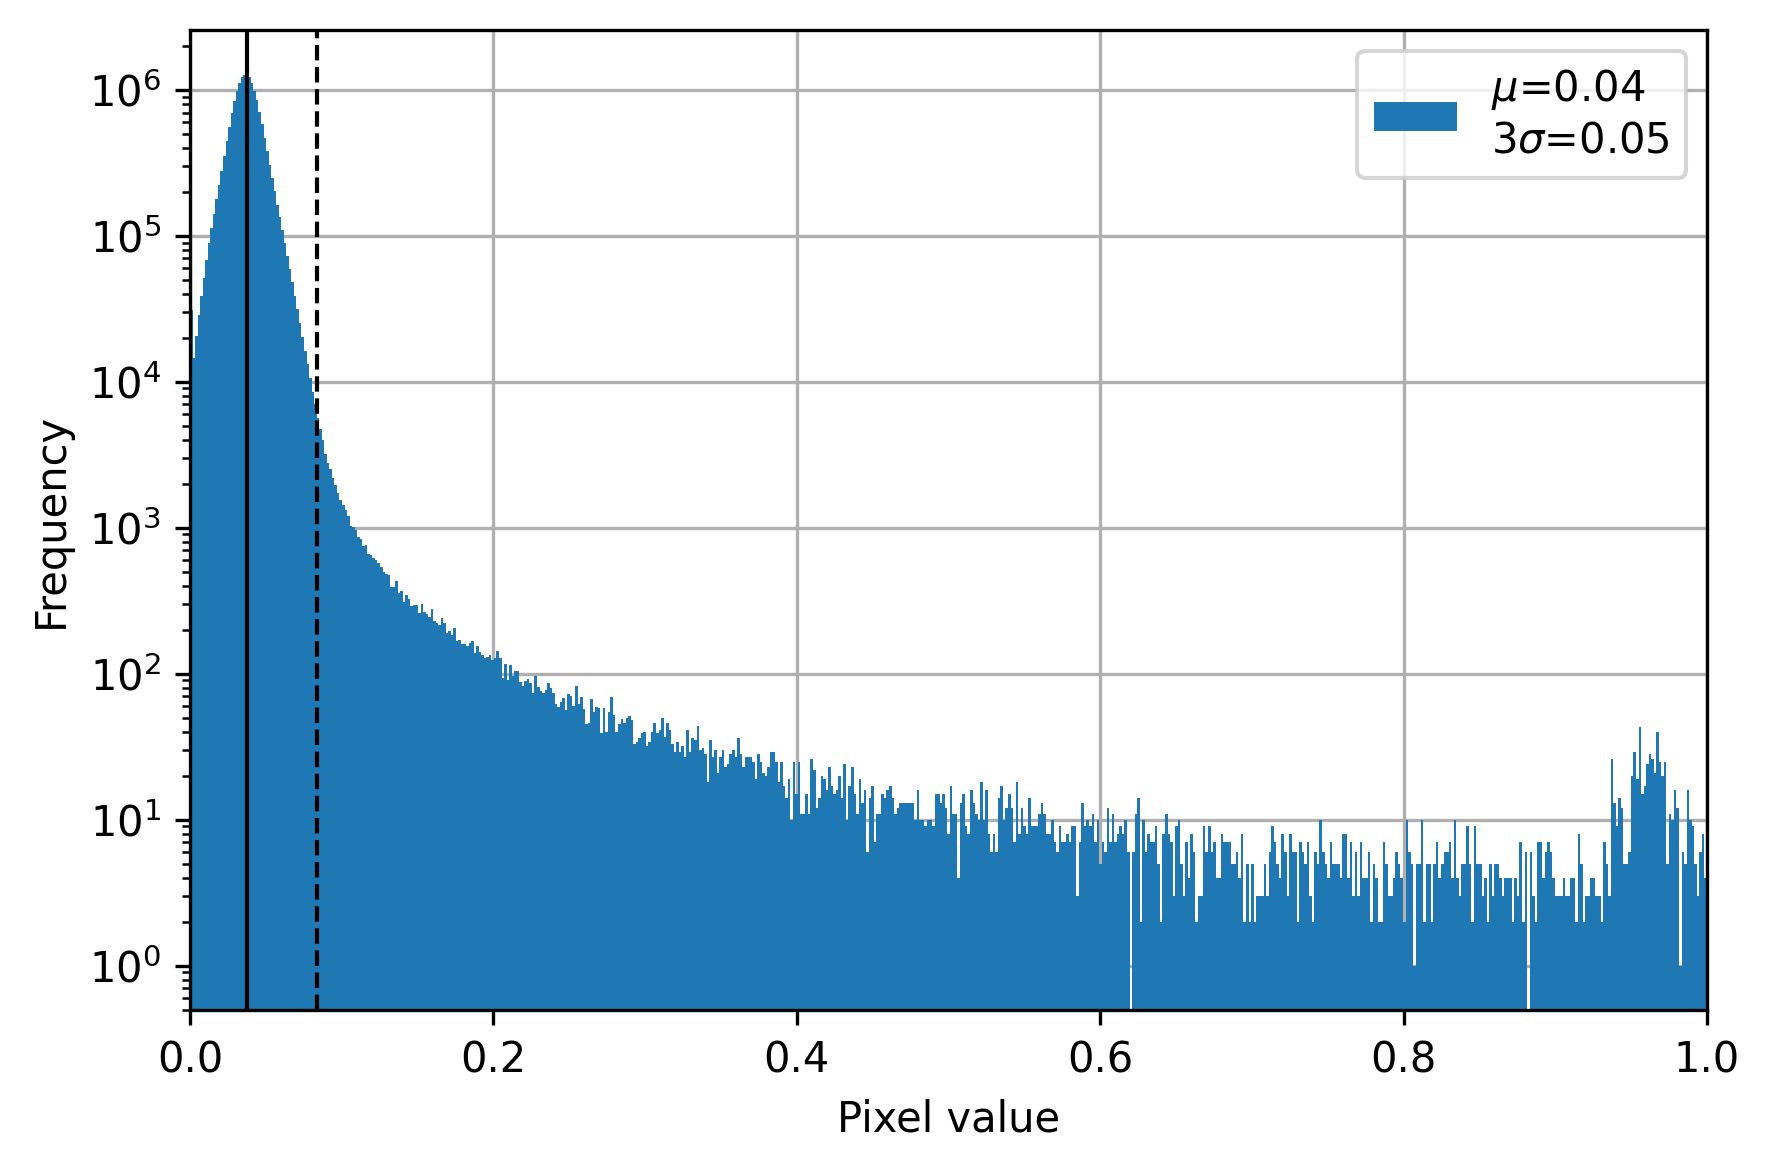
\includegraphics[width=\linewidth]{histogram_output.png}
  %   \caption{Calibrated image\\\text{}}
  %   \label{fig:before-removing-stars}
  % \end{subfigure}%
  % \hfill
  \begin{subfigure}{.49\textwidth}
    \centering
    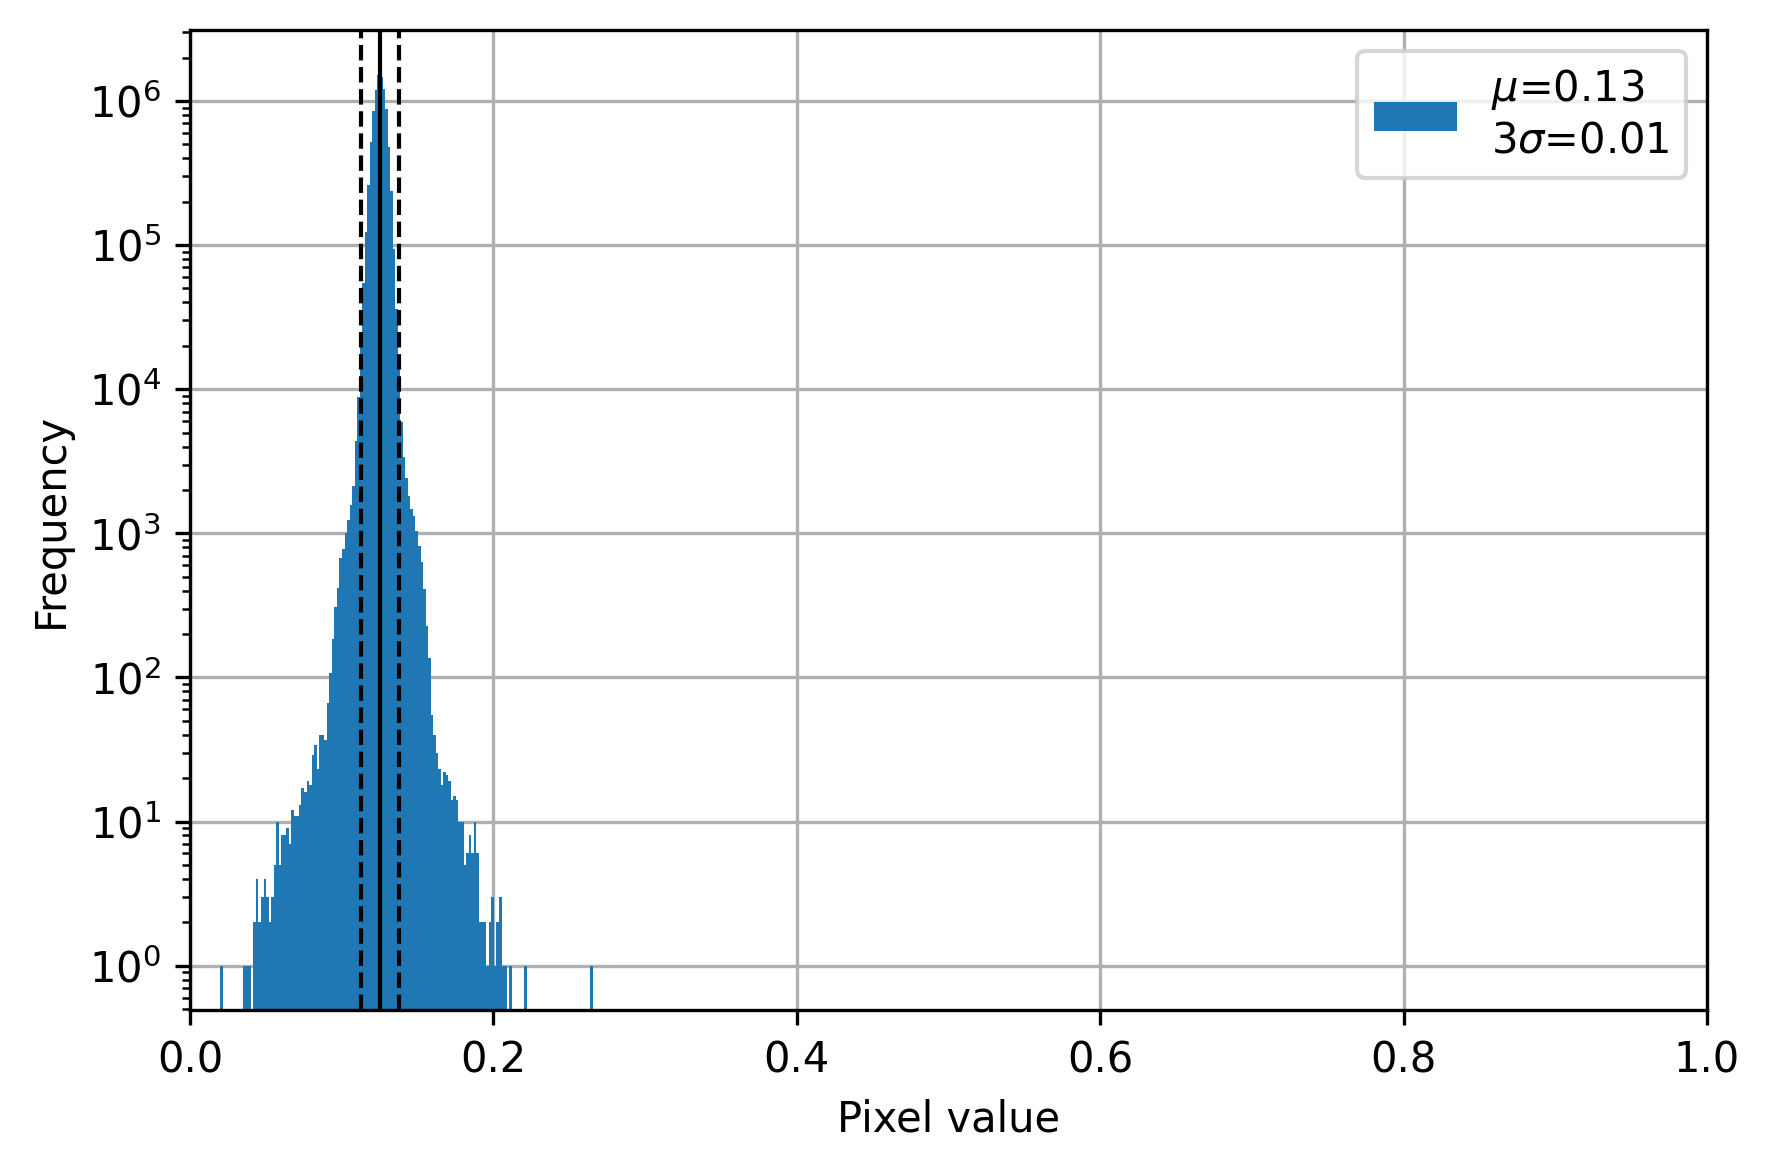
\includegraphics[width=\linewidth]{histogram_black_single.png}
    \caption{Black image taken with the lens cap on, not normalized.}
    \label{fig:black-histogram}
  \end{subfigure}%
  \hfill
  \begin{subfigure}{.49\textwidth}
    \centering
    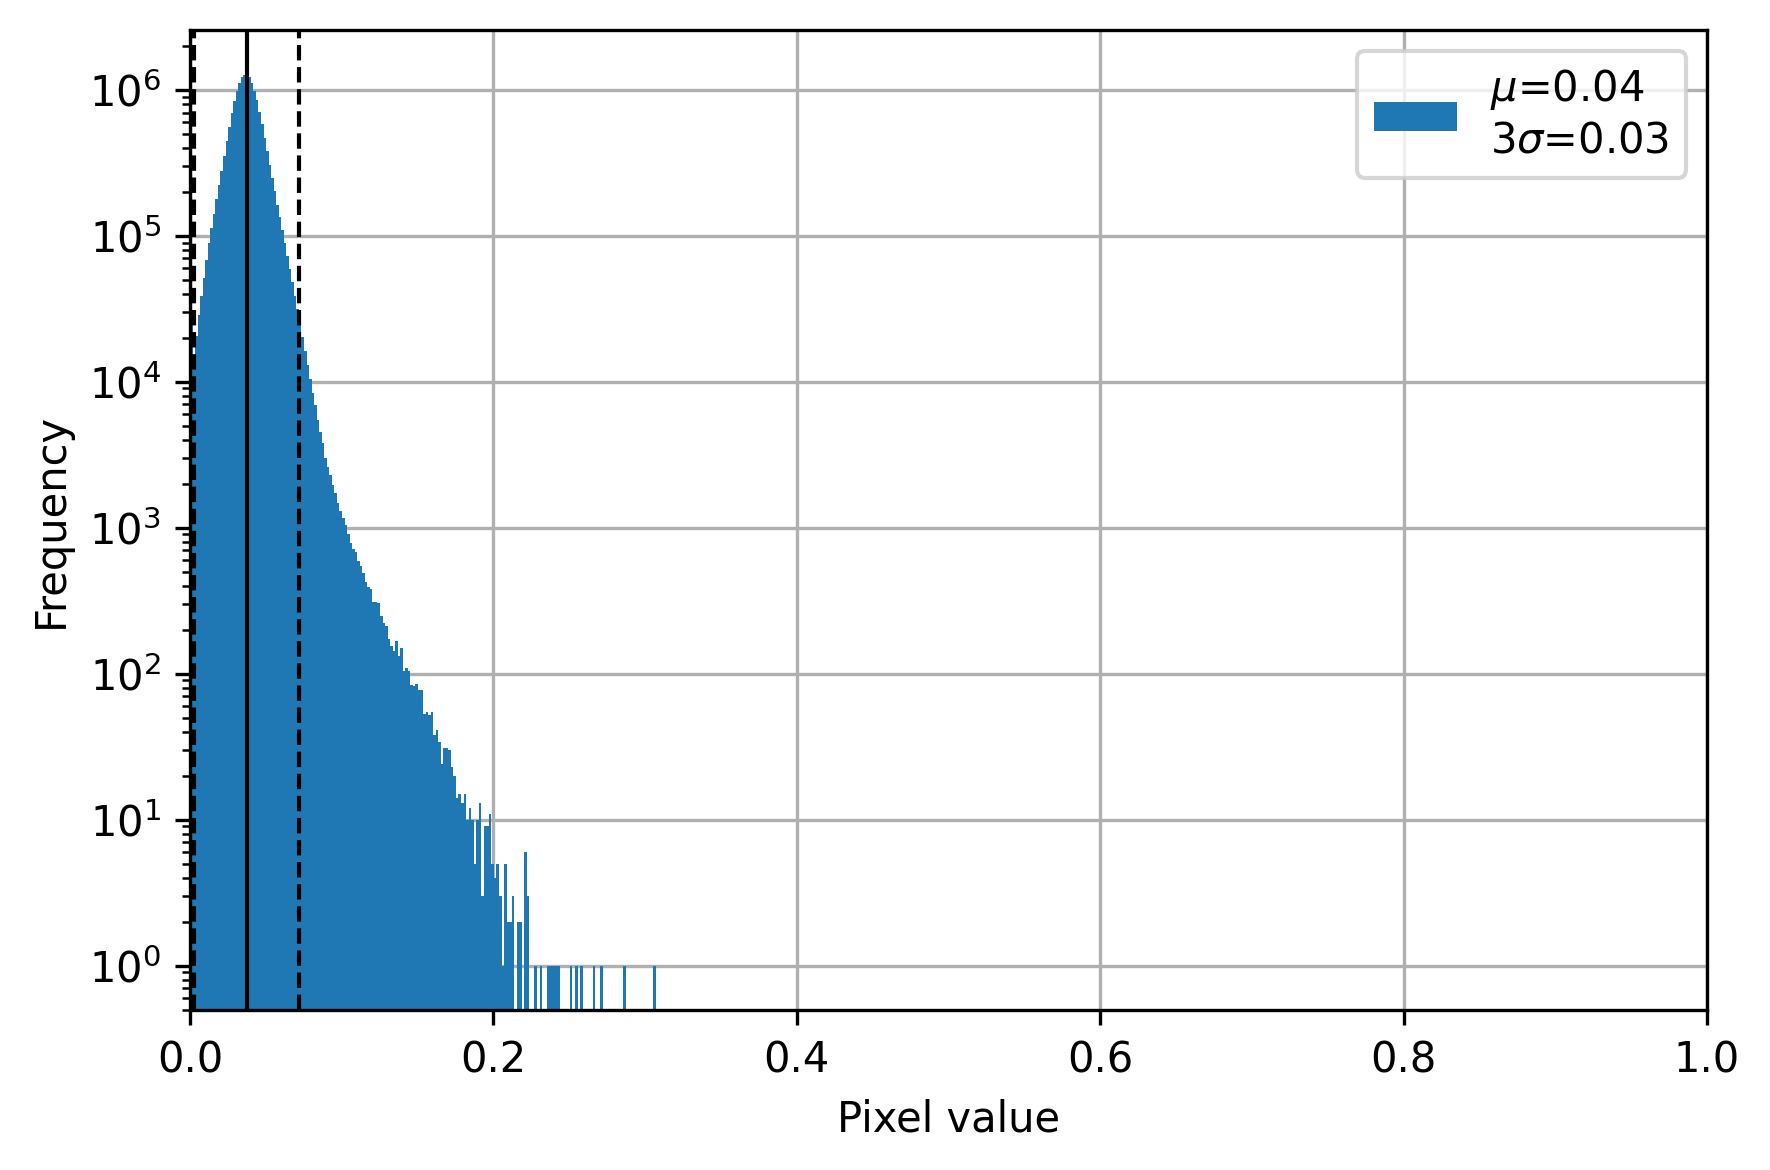
\includegraphics[width=\linewidth]{histogram_no_stars.png}
    \caption{After removing all star-pixels found by the method in \autoref{sec:star-identification}.}
    \label{fig:after-removing-stars}
  \end{subfigure}
  \caption{}
  \label{fig:removing-stars}
\end{figure}

\subsection{Pixel to Sky Mapping}
\label{sec:pixel-to-sky-mapping}

To find the true magnitude of a star in the input image, we need to know its right
ascension and declination. This requires mapping the pixel coordinates of the star to the
celestial sphere. Therefore, we need to know the orientation of the camera and the field
of view of the lens. The website
\href{https://nova.astrometry.net}{\texttt{astrometry.net}} \cite{astrometry2010} allows
users to upload an image and returns the world coordinates of the center of the image and
other helpful information. An upload of the input image is linked and shown in
\autoref{fig:astrometry-output}. However, as the \texttt{brightest} library is meant to be
used without manual intervention or an internet connection, I used the \texttt{astrometry}
Python library, which only includes the algorithm for astrometric plate solving used by
the website. Given a set of pixel coordinates and limits for the field of view, the
\texttt{astrometry} library returns an \texttt{astropy.WCS} (World Coordinate System)
object, which can be used to map pixel to world coordinates.

The solver tries to find the best match between the input coordinates and a catalog of
stars. I used the recommended built-in dataset based on a subset of the Tycho-2 catalog,
available at \href{http://data.astrometry.net/4100/}{\texttt{data.\allowbreak
    astro\allowbreak metry.\allowbreak net}}. Additionally, the solver is given a lower and
upper limit for the scale of the image, expressed in arcseconds per pixel. My camera has a
sensor size of $x \times y = 22.3 \times 14.9$ mm and a focal length of $f = 18$. Then
field of view is given by
\begin{align*}
  \text{FOV}_x & = 2 \arctan{\left(\frac{x}{2f}\right)} = 63.55^\circ  \\
  \text{FOV}_y & = 2 \arctan{\left(\frac{y}{2f}\right)} = 44.97^\circ.
\end{align*}
With a horizontal resolution of 5202 pixels, we get $\text{scale} = \text{FOV}_x / 5202 =
  43.98$ arcsec/pixel. For the input image (\autoref{fig:sky-input}), the solver located
the center of the image at right ascension $20^\text{h}\ 50^\text{m}\ 49.81^\text{s}$
and declination $+60^\circ\ 10'\ 15.02''$. An annotated version of the image, showing
the constellations, is shown in \autoref{fig:astrometry-output}. Using the returned
\texttt{astropy.WCS} object, the pixel coordinates of the stars are transformed to sky
coordinates.

\subsection{Catalog Matching}
\label{sec:catalog-matching}

Now that we know the sky coordinates of the stars in the input image, we can match them
to stars in a catalog provided by the user. As mentioned in
\autoref{sec:pixel-to-sky-mapping}, the \texttt{astrometry} library already provides a
built-in catalog. However, it is only a small subset of the Tycho-2 data so that the
solver can run quickly.

Instead, I queried the SIMBAD database \cite{Wenger_2000}. It is one of the most
comprehensive astronomical databases and presently contains information on about 8.9
million stars and 9.3 million non-stellar objects. I queried the database for stars with a
visible magnitude of less than 8.0 in the field of view of the input image. Visual
inspection showed that stars with a higher magnitude were not distinguishable from noise
in the calibrated image. For other images, the maximum magnitude can be set by the user.

Matching the star positions is done by calling the \texttt{SkyCoord.\allowbreak
  match\_to\_catalog\_sky} method from the \texttt{astropy} library \cite{astropy2022} with
the sky coordinates of the stars in the image and the catalog. It constructs a KD-Tree
from the catalog and performs a nearest-neighbor search for each star in the image. The
result is an index map that assigns a catalog star to each star in the image. The accuracy
of this method depends mostly on the accuracy of the solution of the astrometric plate
solver (\autoref{sec:pixel-to-sky-mapping}). The more the coordinates are off, the higher
the chance that the nearest neighbor is not the correct match. Therefore, it is important
to use a conservative maximum magnitude for the SIMBAD query to keep the size of the
catalog close to the number of stars in the image.

\subsection{Magnitude Estimation}
\label{sec:magnitude-estimation}

\begin{figure}[tb]
  \centering
  \begin{subfigure}{.49\textwidth}
    \centering
    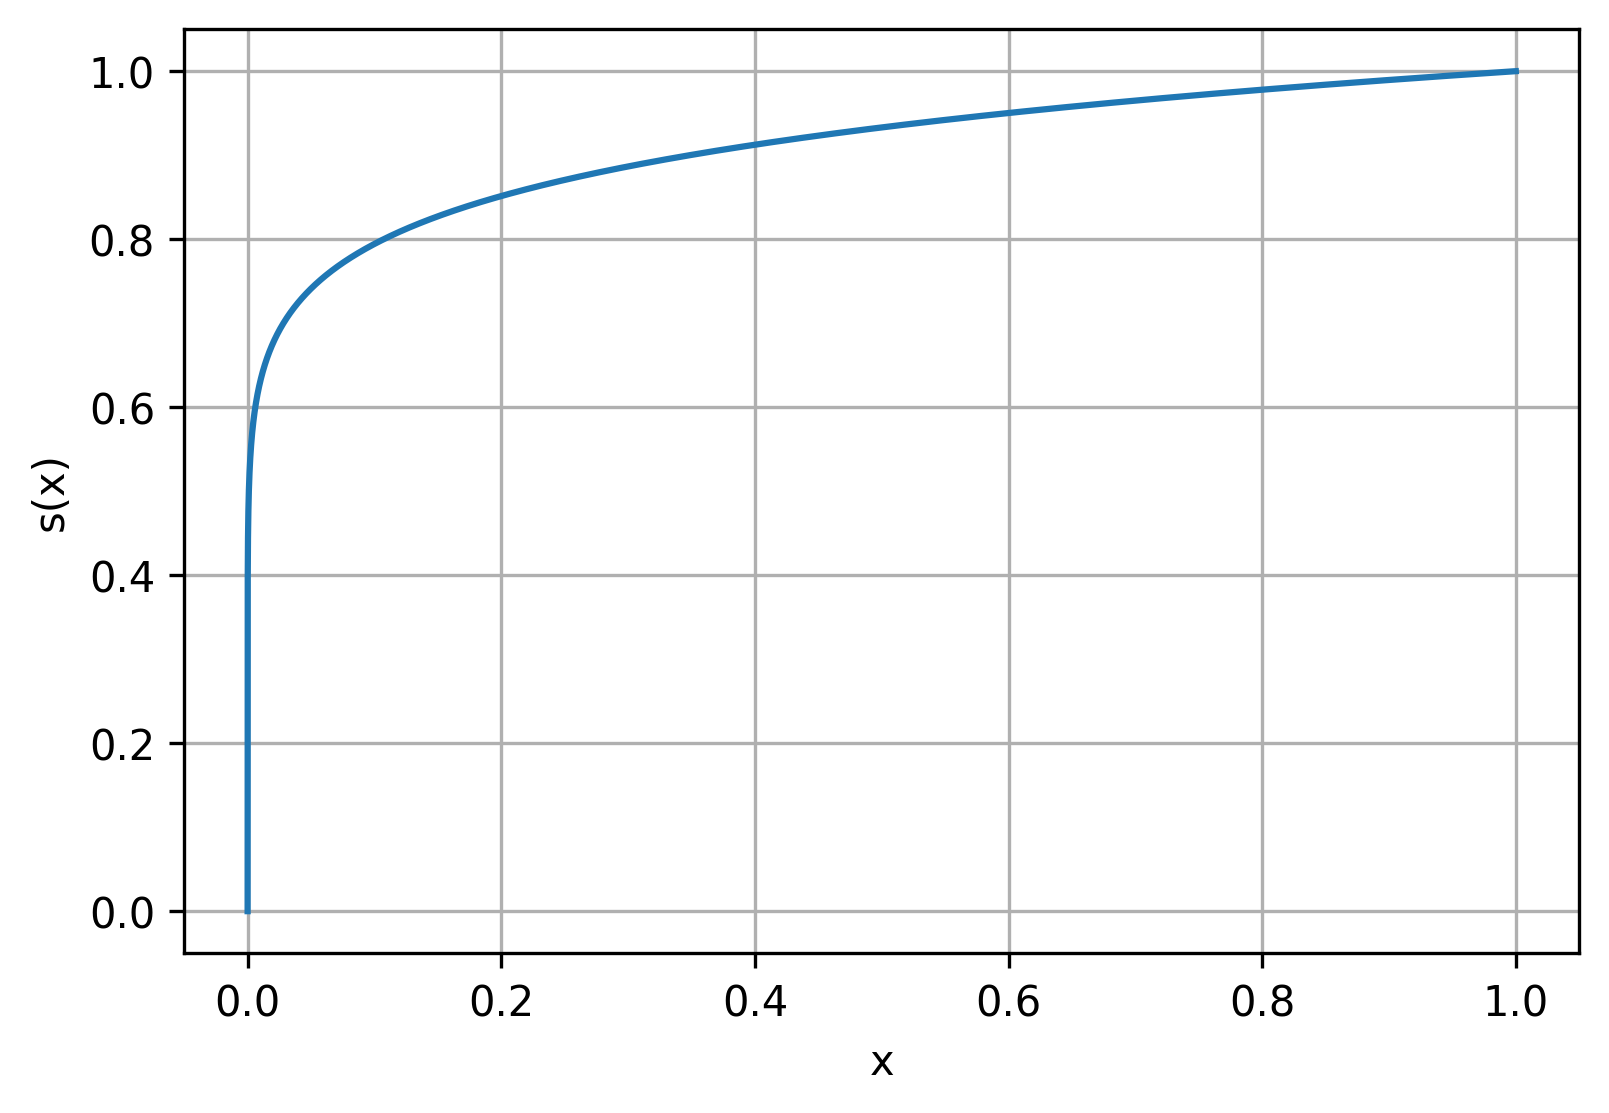
\includegraphics[width=\linewidth]{x_pow_0.1.png}
    \caption{Scaling function $s(x) = x^{0.1}$}
    \label{fig:kmeans-scaling}
  \end{subfigure}%
  \hfill
  \begin{subfigure}{.49\textwidth}
    \centering
    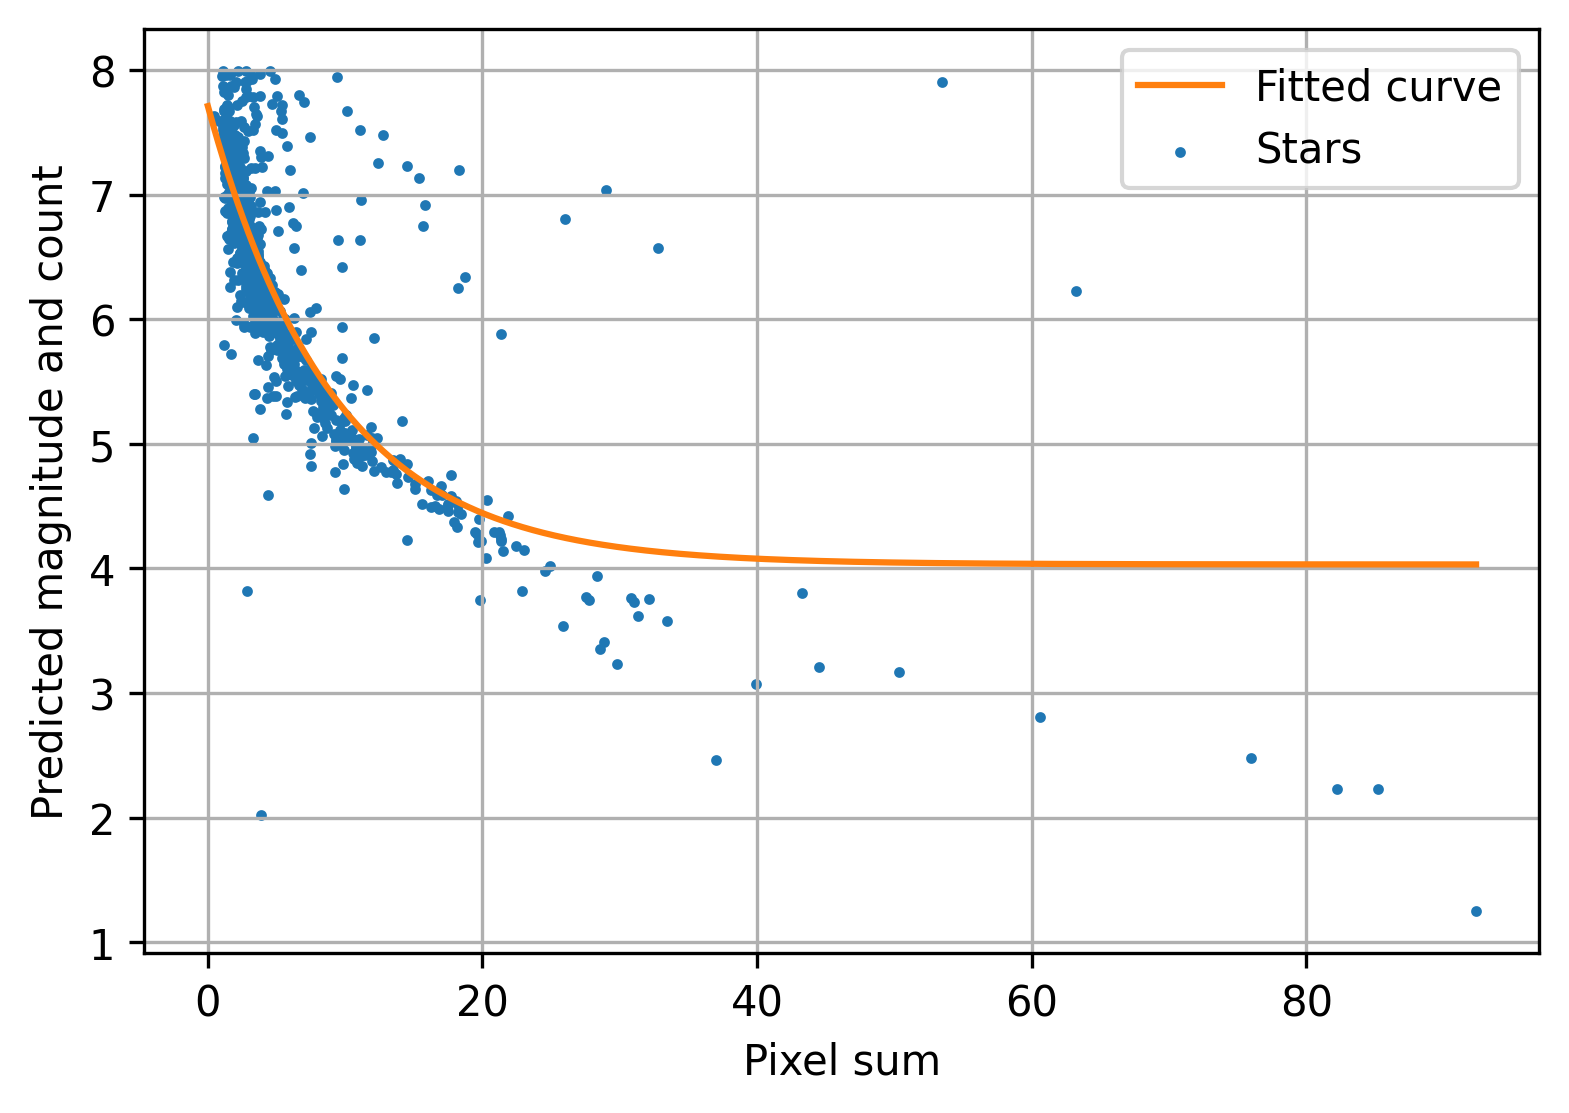
\includegraphics[width=\linewidth]{histogram_fitted.png}
    \caption{Fitted exponential function $f(x)$}
    \label{fig:fitted-exponential}
  \end{subfigure}
  \caption{}
\end{figure}

The magnitude of a star is a measure of the intensity of light it emits on a reverse
logarithmic scale. We want to predict the magnitude of the stars in the image for further
analysis. The pixel mask that was created in \autoref{sec:star-identification} gives us a
set of pixels with values in $[0, 1]$ for each star. This serves as the basis for the
estimation and will be summed up to get the total intensity of the star. As the
\texttt{floodFill} method selects pixels based only on the intensity difference to their
direct neighbors, the selection of pixels with a medium value is inconsistent.

\begin{figure}[tb]
  \centering
  \begin{subfigure}{.49\textwidth}
    \centering
    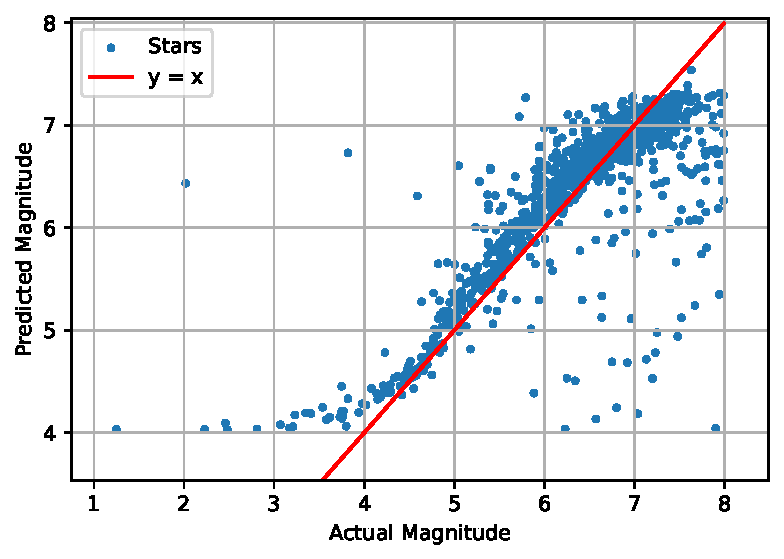
\includegraphics[width=\linewidth]{magnitude_prediction.pdf}
    \caption{Prediction with the exponential function $f(x)$}
    \label{fig:prediction-exponential}
  \end{subfigure}%
  \hfill
  \begin{subfigure}{.49\textwidth}
    \centering
    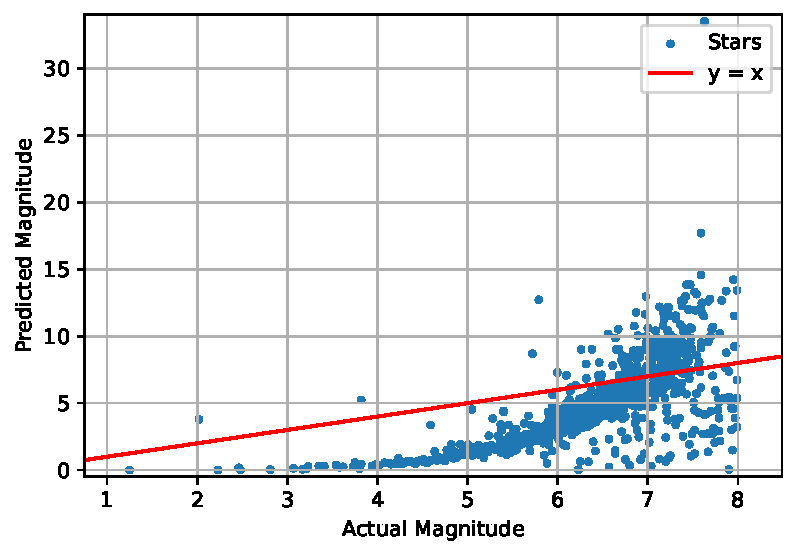
\includegraphics[width=\linewidth]{magnitude_prediction_log.pdf}
    \caption{Prediction with the logarithmic function $g(x)$}
    \label{fig:prediction-logarithmic}
  \end{subfigure}
  \caption{Comparison of the predicted magnitudes to the true magnitudes.}
  \label{fig:prediction}
\end{figure}

To get a more accurate selection, I first scaled the image using the function $s(x) =
  x^{0.1}$ (see \autoref{fig:kmeans-scaling}). This spreads out the values of the dimmer
pixels to make them more distinguishable. Then, I applied k-means clustering with $k =
  2$ to the pixels within the bounding box of each star. Pixels belonging to the cluster
with the higher mean are considered star-pixels, and background-pixels otherwise. The
clustering separates bright from dark pixels more consistently without any predefined
factor or shape. I chose centroid-based clustering, because it can guarantee two
clusters. For the implementation, I used the \texttt{KMeans} class from the
\texttt{scikit-learn} library \cite{scikit-learn}.

After refining the mask, I fitted an exponential function to the data. It takes the sum of
pixels, that were classified as star-pixels, as input and returns the magnitude. The
function is defined as
\begin{align*}
  f(x) = a \cdot \exp{\left(-b \left(\frac{x}{30} - c\right)\right)} + d,
\end{align*}
where $a$, $b$, $c$ and $d$ are the parameters to be fitted. The factor $30$ is used to
ensure convergence of the optimization algorithm. The parameters are fitted using the
\texttt{curve\_fit} method from the \texttt{scipy} library \cite{scipy2020}. The optimal
values of the parameters are $a = 0.47$, $b = 3.28$, $c = 0.63$ and $d = 4.03$ and the
resulting function is shown in \autoref{fig:fitted-exponential}.

I tested other functions, like a polynomial, hyperbolic, logarithmic and variations of
trigonometric functions. The function $g(x) = a \cdot \log(1 / x + b)$ would be the most
appropriate in the physical sense, as it is a convex function with $\lim_{0 \leftarrow x}
  g(x) = \infty$ which can produce negative values. However, having many points with a low
pixel sum meant that the fitted function assigned the same magnitude to all brighter
stars. A comparison of the magnitude predicted by the logarithmic function to the true
magnitudes is shown in \autoref{fig:prediction-logarithmic}. I settled on the exponential
function (\autoref{fig:fitted-exponential}) mentioned above, because it produced the
lowest mean squared error. For a pixel sum of 0, the function returns a magnitude of
$7.5$, which is the maximum magnitude of the stars in the image. Any star with a higher
magnitude is not distinguishable from noise. The function stagnates towards a magnitude of
$4$ from a pixel sum of $50$ onwards. This is likely due to a lack of training data and
saturation of the sensor for a majority of the pixels.

The mean squared error of the fit without the clustering step was $0.366$. With the
clustering, but without the scaling by $s(x)$, the error was $0.349$. The final error
after applying both mask refinement steps was $0.334$, which is a reduction of $9.6\%$
compared to the initial error. The MSE of the logarithmic function $g(x)$ was $0.452$. A
comparison of the predicted magnitudes to the true magnitudes is shown in
\autoref{fig:prediction}. The true magnitudes are on the x-axis and the predicted
magnitudes on the y-axis, with the red line $y = x$ for reference. The function is not
perfect, but it is a good approximation for the majority of stars. The outliers could be
due to the stars being matched to the wrong catalog star or two stars being recognized as
one object. Also, very bright stars are not estimated well, likely because they are
saturated in the image.

\subsection{Source-Count Distribution}
\label{sec:source-count-distribution}

A source-count distribution is a cumulative distribution of the number of sources ($N$)
brighter than a given flux density ($S$). It corresponds to the volume integration of
those stars which generate a received radiation flux of $S > S_0$ for a given flux density
$S_0$. Using the distance-luminosity relation $L(S) = 4 \pi r^2 S$, where $r$ is the
distance to the source, and integrating over the luminosity function $\Phi(L)$, we can
derive the general form of the source-count distribution as
\begin{align*}
  N(> S) = N_0 \cdot \left(\frac{S}{S_0}\right)^{-\frac{3}{2}},
\end{align*}
where $N_0$ and $S_0$ are normalization constants. The slope of the distribution is
determined by the power-law index -3/2. With the definition of the magnitude $m - m_0 =
  -2.5 \log_{10}{(S/S_0)}$, we can express the source-count distribution in terms of the
magnitude as
\begin{equation}
  \log_{10}{(N(< m))} = \log_{10}{(N_0)} + 0.6 \cdot (m - m_0).
  \label{eq:source-count}
\end{equation}
We can use this relation to verify the accuracy of the magnitude estimation. The
distribution of the magnitudes of the stars in the calibrated image, estimated by the
approach in \autoref{sec:magnitude-estimation}, is shown in
\autoref{fig:distribution-predicted}. For comparison, the same plot is shown for the stars
obtained from the SIMBAD database using the query in \autoref{lst:simbad-query} in
\autoref{fig:distribution-true}. I fitted the function in \autoref{eq:source-count} to the
cumulative distribution, with the slope, $N_0$ and $m_0$ as free parameters. From the fit,
I obtained a slope of $0.41$ for the predicted magnitudes and $0.51$ for the true
magnitudes, which is close to the expected value of $0.6$. One of the main reasons for the
deviation is likely the low accuracy of the predictor for bright stars. As no star
receives a magnitude of less than $4$, the distribution is inflated at the bright end,
which contributes to the lower slope. Also, the distribution would likely approach a slope
of $0.6$ more closely, if the distribution would include stars with a magnitude higher
than 8.0. I suspect this is the reason for the lower slope of the true magnitudes as well.

\begin{figure}[tb]
  \centering
  \begin{subfigure}{.49\textwidth}
    \centering
    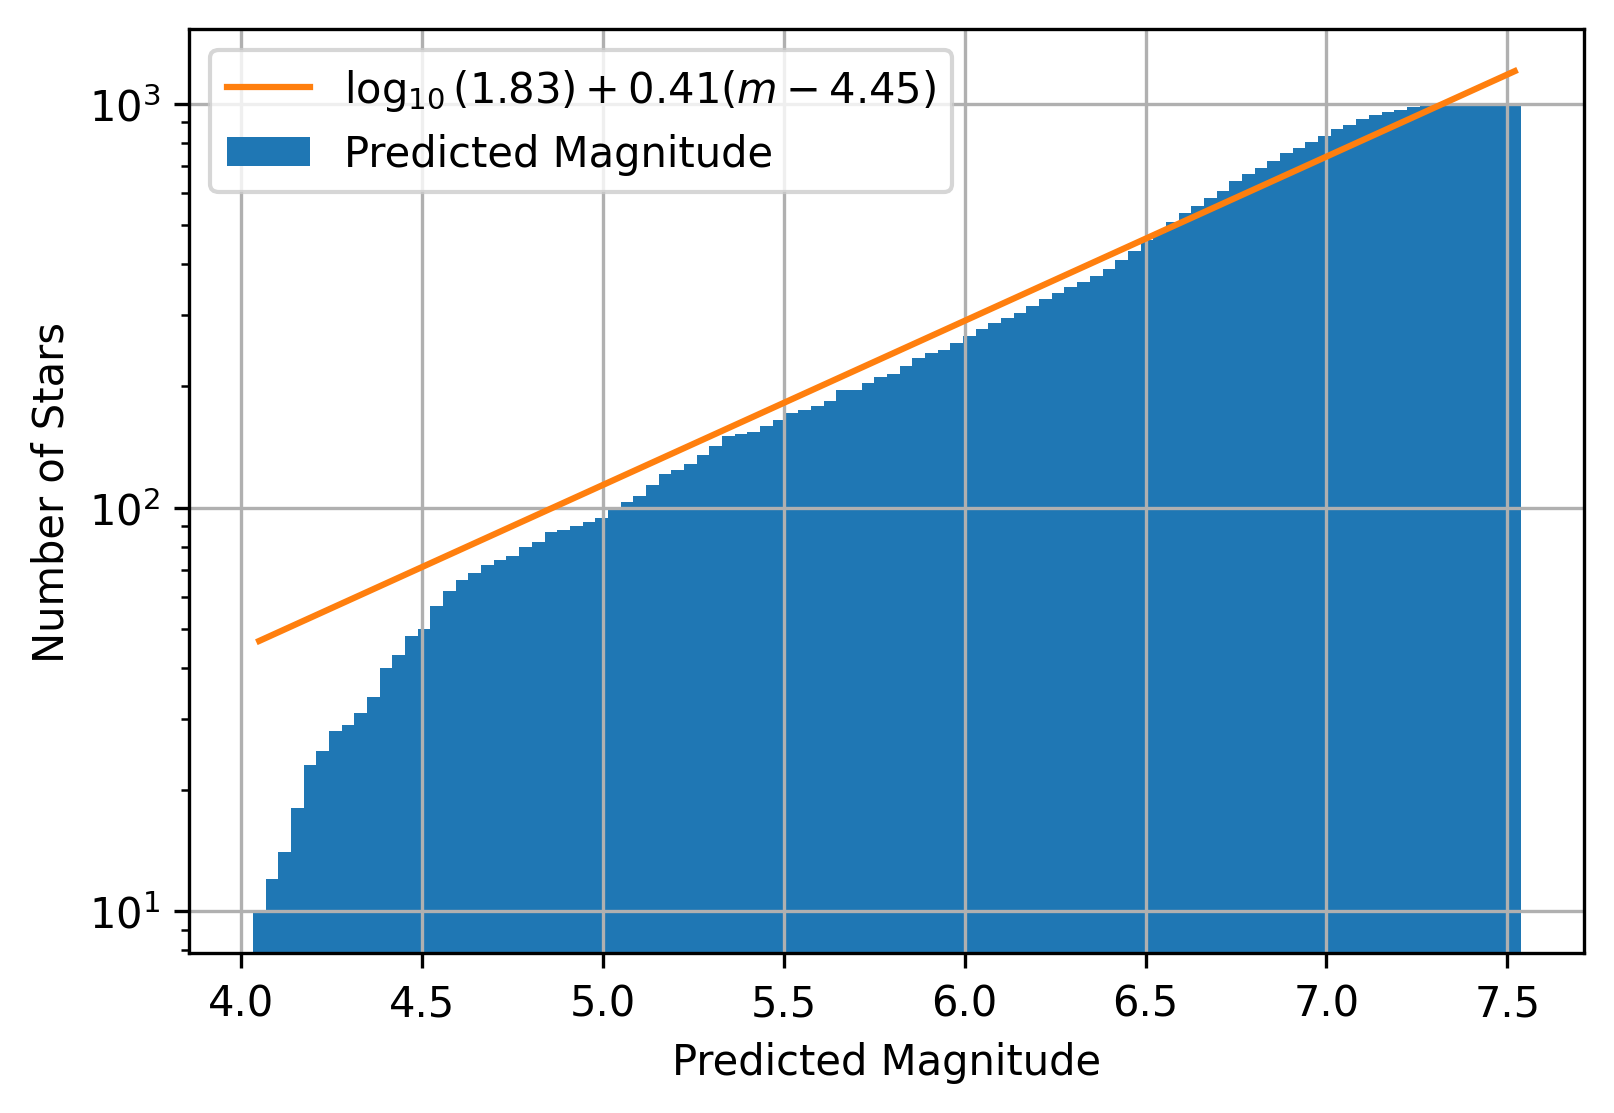
\includegraphics[width=\linewidth]{source_count_predicted.png}
    \caption{Prediction with the exponential function $f(x)$}
    \label{fig:distribution-predicted}
  \end{subfigure}%
  \hfill
  \begin{subfigure}{.49\textwidth}
    \centering
    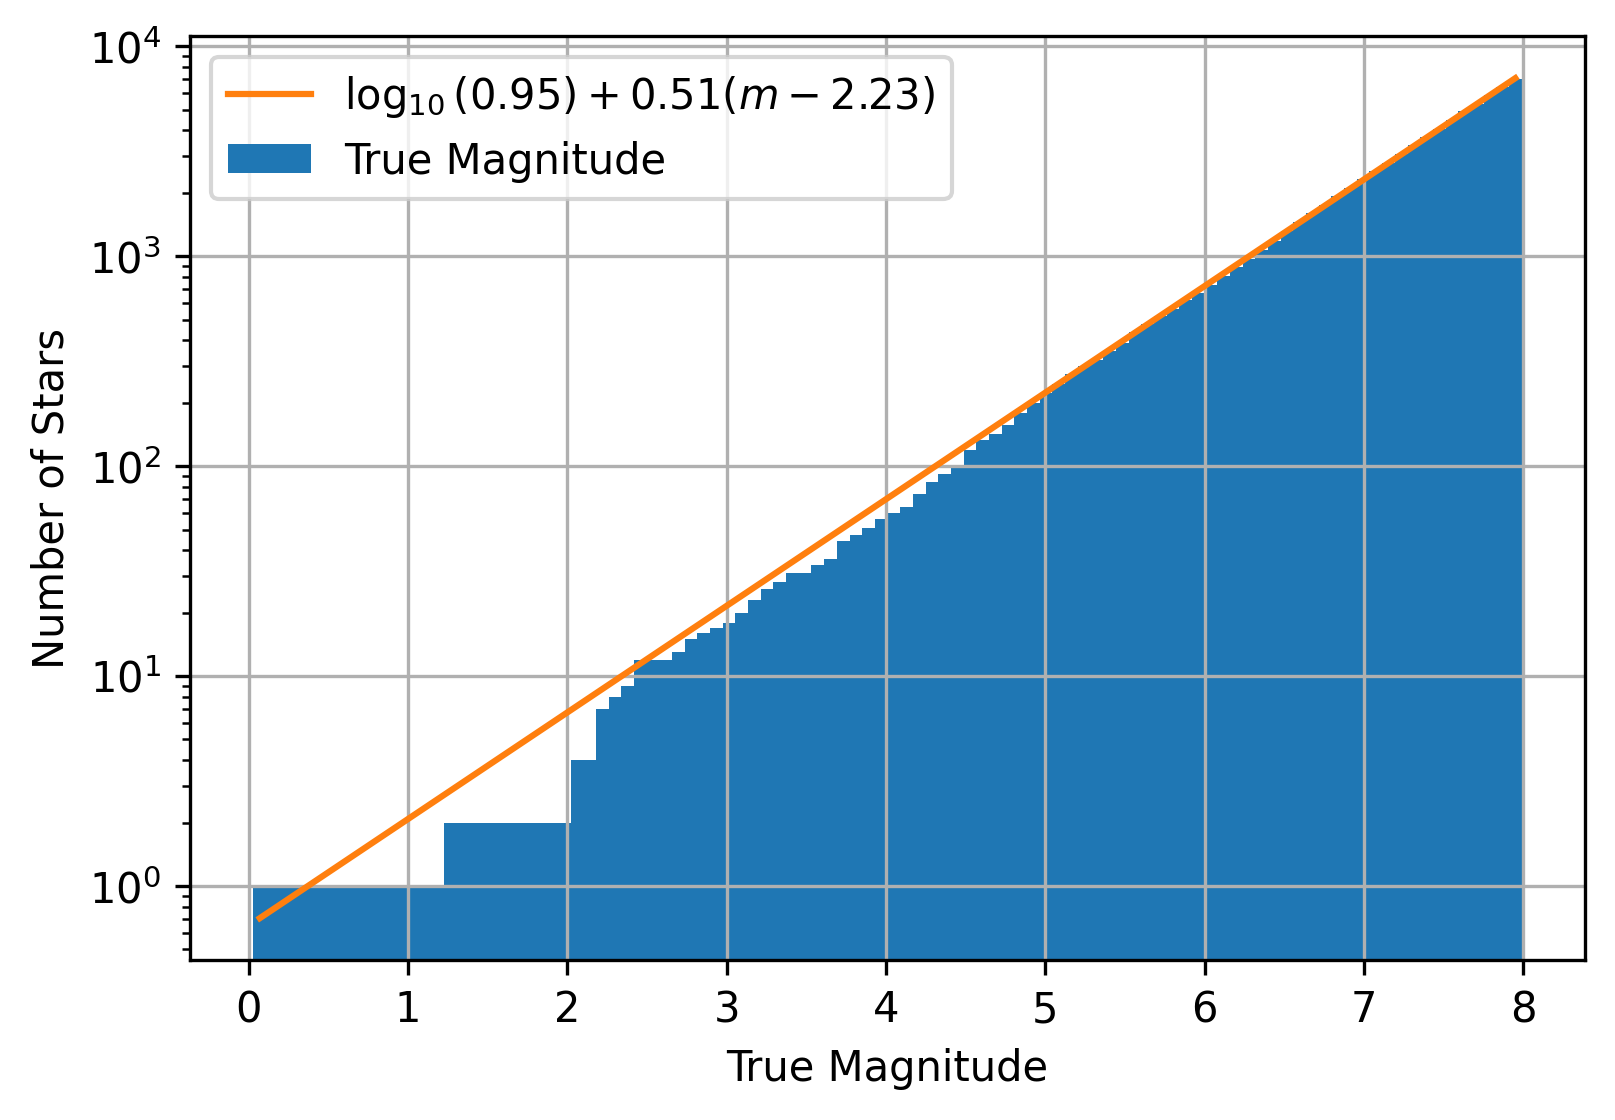
\includegraphics[width=\linewidth]{source_count_true.png}
    \caption{Prediction with the logarithmic function $g(x)$}
    \label{fig:distribution-true}
  \end{subfigure}
  \caption{}
  \label{fig:source-count}
\end{figure}
